

%!TEX root = ../Notes.tex
\section{Covering Maps}

Our ultimate goal is to find a space with an interesting fundamental group. 
\begin{definition}
	Let $X$ and $\widetilde{X}$ be topological spaces, and $p:\widetilde{X}\twoheadrightarrow X$ be a continuous surjection. An open set $U \subseteq X$ is said to be \textbf{evenly covered} by $p$ if $p^{-1}(U)$ is the disjoint union of open sets $V_{\alpha}$, $\alpha \in A$ for some index set $A$, such that for all $\alpha \in A,$ $p \mid V_{\alpha} \rightarrow U$ is a homeomorphism. 
	
	In this case, we say that each $V_{\alpha}$ is a \textbf{sheet} covering $U$. 
\end{definition}
\begin{example}
	Let $X=D^2$ with the usual topology, and $\widetilde{X}=D^2 \times \N$ with the usual product topology. Define $p:\widetilde{X} \rightarrow X$ by $p(x,n)=x.$ We can take $U$ to be any open set in $X$; $\displaystyle p^{-1}(U)=\bigcup_{i=1}^{\infty}p^{-1}(U)\cap V_i$, where $V_i=D^2 \times i$.
	
	\[ 
	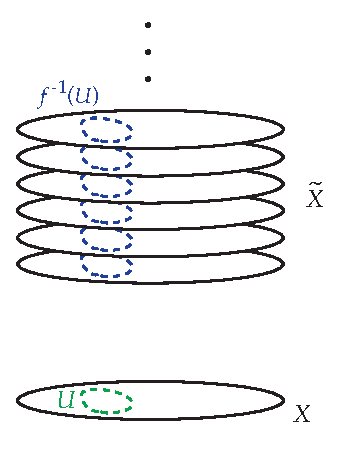
\includegraphics[width=150pt]{images/covering_spaces/D2xN} \]
\end{example}
\begin{example}
	[a non-example] Let $\widetilde{X}=S^1,$ and let $X=S^1 \lor S^1.$ That is, $X$ is two copies of $S^1,$ which agree at a point. 
	
	Let $\sim$ be the equivalence relation on $S^1$ given by $x \sim y$ if and only if $x,y \in \{x_1,x_2\}$ or $x=y$. Let $p$ the the quotient map from $\widetilde{X}$ to $X$, corresponding to this relation, and let $U$ be an open set in $X$ containing $x_1,x_2,$ as shown. Is $U$ evenly covered?
	
	The answer is no. To see why, note that $p^{-1}(U)=V_1 \cup V_2,$ where $V_1,V_2$ are disjoint open sets in $\widetilde{X}$. But $p \vert V_1: V_1 \rightarrow U$ is not a homeomorphism because it is not onto. 
\end{example}
\begin{definition}
	Let $p: \widetilde{X} \twoheadrightarrow X$ be a continuous surjection. Suppose for all $x \in X$, there exists an evenly covered open set $U$ containing $X$. We say $p$ is a \textbf{covering map}, $\widetilde{X}$ is the \textbf{covering space} and $X$ is the \textbf{base space.} 
\end{definition}
\begin{example}
	[another non-example] Let $\widetilde{X}=\R^2,$ $X=\R,$ and $P:\R^2\rightarrow \R$ be defined by $p(x,y)=x$. Then for each open $U \subseteq X,$ $p^{-1}(U)=\cup_{\alpha \in A}V_{\alpha}.$ (We can think of $p^{-1}(U)$ as a horizontal stack of uncountably many copies of $U$). For each $\alpha \in A,$ $p \mid V_{\alpha}: V_{\alpha} \rightarrow U$ is a homeomorphism. However, each $V_{\alpha}$ is not open in $\widetilde{X}$. 
\end{example}
\begin{lemma}
	[Important Lemma on Covering Maps] Let $p:\widetilde{X} \rightarrow X$ be a covering map. Let $x \in X$. Then the subspace topology on $p^{-1}(\{x\})$ is the discrete topology. 
\end{lemma}
\begin{proof}
	Let $y \in p^{-1}(\{x\}).$ We want to show that $\{y\}$ is open in $p^{-1}(\{x\})$. Since $p$ is a covering map, there exists a evenly covered open set $U$ containing $x$. Then $p^{-1}(U)=\cup_{\alpha \in A}V_{\alpha}$, where the $V_{\alpha}$ are pairwise-disjoint open sets such that $p \mid V_{\alpha}:V_{\alpha}\rightarrow U$ is a homeomorphism for every $\alpha \in A$. Hence, there exists $\alpha_0 \in A$ such that $y \in V_{\alpha_0}$. Now, $V_{\alpha_0}$ is open in $\widetilde{X}$. Note that $y \in V_{\alpha_0}\cap p^{-1}(\{x\})$. Let $y' \in V_{\alpha_0} \cap p^{-1}(\{x\})$ be given. We know that $p \mid V_{\alpha_0}$ is a homeomorphism, so it is injective. Since $p(y')=x,$ and $p(y)=x,$ we see that $y=y'$. Thus, $\{y\}=V_{\alpha_0} \cap p^{-1}(\{x\})$, both of which are open in $p^{-1}(\{x\}).$ So $\{y\}$ is open in $p^{-1}(\{x\})$ with the subspace topology. This completes the proof. 
\end{proof}

The take-home message is that in a covering space, points in the pre-image of a single point are ``spread out."
\begin{example}
	[Important] Let $p:\R \rightarrow S^1$ be defined by $p(x)=(\cos(2 \pi x), \sin(2 \pi x))$. (The ``slinky" space.)
	
	\[ 
	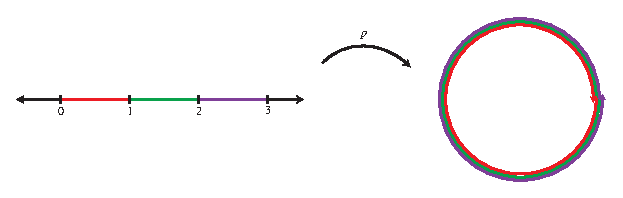
\includegraphics[width=330pt]{images/covering_spaces/slinky} \]
	
	For each $s \in S^1,$ an ``open interval" around $s$ is evenly covered, and so $\R$ is a covering space. 
\end{example}
\begin{example}
	$\widetilde{X}=S^1,$ $X=S^1$ by $p:\widetilde{X} \rightarrow X$ is $p((\cos(2 \pi x), \sin(2\pi x))=(\cos(4 \pi x), \sin(4 \pi x)).$ 
	
	\[ 
	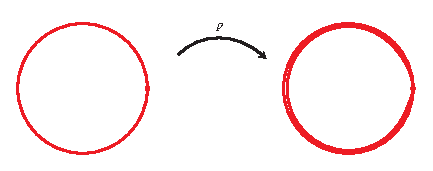
\includegraphics[width=330pt]{images/covering_spaces/s1_to_s1_new} \]
\end{example}

Not all quotient maps are covering maps. But we will prove that all covering maps are quotient maps. (Remember our important example?)
\begin{theorem}
	Let $p:\widetilde{X}\rightarrow X$ be a covering map. Then 
	\begin{enumerate}
		\item $p$ is an open map 
		\item $X$ is a quotient space, and $p$ is a quotient map. 
	\end{enumerate}
\end{theorem}
\begin{proof}
	Let $U$ be open in $\widetilde{X}$. We want to show that $p(U)$ is open. Let $x \in p(U).$ Then there exists an evenly covered open set $V$ containing $X$. Now, there exists $y \in U$ such that $p(y)=x.$ Then $p^{-1}(V)=\cup_{\alpha \in A}V_{\alpha}$ such that the $V_{\alpha}$ are disjoint open sets and $p \mid V_{\alpha}$ is a homeomorphism for all $\alpha \in A$. Let $\alpha_0 \in A$ such that $y \in V_{\alpha_0}$. There exists such an $\alpha_0$ because $x \in V$.
	
	Because $U$ and $V_{\alpha_0}$ are both open, $U\cap V_{\alpha_0}$ is open in $\widetilde{X}$. Recall $p\mid V_{\alpha_0}:V_{\alpha_0}\rightarrow V$ is a homeomorphism, so 
	\begin{align*}
		p(U\cap V_{\alpha_0})&=p\left(V_{\alpha_0}\cap p(U)\right)\\
		&=V\cap p(U) 
	\end{align*}
	where $V\cap p(U)$ is open in $V$ and $U$ is open in $X$. Therefore, $V\cap p(U)$ is open in $X$. Because our $x$ is in both $V$ and $p(U)$, $x\in V\cap p(U)\subseteq p(U)$. That is, $x$ is an element of an open set contained in $p(U)$. Hence, $p(U)$ is open and $p$ is an open map. 
	\item To show $X$ has the quotient topology with regard to $p$, we want to show that $F_X = \{U\subseteq X \mid p^{-1}(U)\in F_X\}$.
	\begin{itemize}
		\item[$(\subseteq)$] Let $V\in F_X$. Because $p$ is continuous, $p^{-1}(V)\in F_{\widetilde{X}}$. Thus, $V\in \{U\subseteq X \mid p^{-1}(U)\in F_X\}$.
		
		\item[$(\supseteq)$] Let $U\subseteq X$ such that $p^{-1}(U)\in F_{\widetilde{X}}$. Because $p$ is open, $p(p^{-1}(U)$ is open in $X$. Because $p$ is onto $p(p^{-1}(U))=U$. Thus, $U\in F_X$. 
	\end{itemize}
	
	$F_X = \{U\subseteq X \mid p^{-1}(U)\in F_X\}$, so $p$ is a quotient map and $X$ is a quotient space. 
\end{proof}

\subsection{Lifts} 
\begin{definition}
	Let $p:\widetilde{X}\rightarrow X$ be a covering map and $f:Y\rightarrow X$ be continuous. We define a \textbf{lift} of $f$ to be any continuous function $\widetilde{f}:Y\rightarrow X$ such that $p\circ \widetilde{f}=f$. 
\end{definition}
\begin{example}
	Let $\widetilde{X}=\R$, $X=S^1$ and $p(x)=\left(\cos(2\pi x),\sin(2\pi x)\right)$. Let $f:I\rightarrow S^1$ by $f(x)=\left(\cos(\pi x),\sin(\pi x)\right)$. Define $\widetilde{f}:I\rightarrow \R$ by $f(x)=\frac{x}{2}$. Then $\widetilde{f}$ is a lift of $f$.
	
	\[ 
	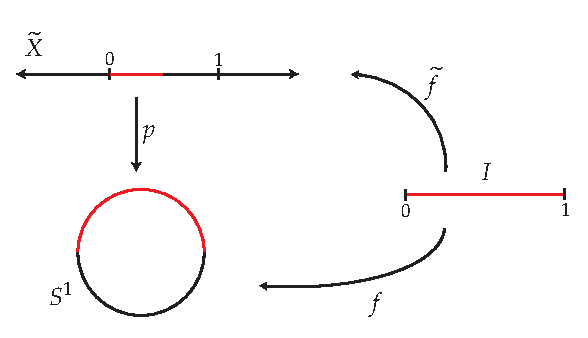
\includegraphics[width=300pt]{images/covering_spaces/s1_lift} \]
\end{example}
\begin{lemma}
	\textbf{Uniqueness of Lifts.} Let $p:\widetilde{X}\rightarrow X$ be a covering map and $f:Y\rightarrow X$ be a covering and $f:Y\rightarrow X$ be continuous and $Y$ be connected. Let $\widetilde{f_0}$ and $\widetilde{f_1}$ be lifts of $f$. Suppose there exists $y_0\in Y$ such that $\widetilde{f_0}(y_0)=\widetilde{f_1}(y_0)$ then $\widetilde{f_0}=\widetilde{f_1}$. 
\end{lemma}
\begin{proof}
	Let $Y' =\{y\in Y\mid \widetilde{f_0}(y)=\widetilde{f_1}(y)\}$. $Y\ne\emptyset$. We want to show that $Y' = Y$, we will accomplish by showing $Y'$ is clopen in $Y$. 
	\begin{itemize}
		\item[Open:] Let $y\in Y'$. There exists an evenly covered open set $V$ containing $f(y)$. $p^{-1}(V)=\displaystyle\bigcup_{\alpha\in A} V_\alpha$ such that $V_{\alpha}$'s are disjoint and open; also, $p\mid V_\alpha:V\alpha\rightarrow V$ is a homeomorphism. 
		
		Let $q= \widetilde{f}_0(y)=\widetilde{f_1}(y)$. There exists and $\alpha_0\in A$ such that $q\in V_{\alpha_0}$. $\widetilde{f}_0^{-1}(V_{\alpha_0})$ and $\widetilde{f}_1^{-1}(V_{\alpha_0})$ are open in $Y$, and $y\in \widetilde{f}_0^{-1}(V_{\alpha_0})\cap\widetilde{f}_1^{-1}(V_{\alpha_0})$. We claim that $\widetilde{f}_0^{-1}(V_{\alpha_0})\cap\widetilde{f}_1^{-1}(V_{\alpha_0})\subseteq Y'.$
		
		Let $z\in \widetilde{f}_0^{-1}(V_{\alpha_0})\cap\widetilde{f}_1^{-1}(V_{\alpha_0}),$ implying $\widetilde{f_0}(z)\in V_{\alpha_0}$ and $\widetilde{f_1}(z)\in V_{\alpha_0}$. Because $\widetilde{f_0}(z)$ and $\widetilde{f_1}(z)$ are lifts of $f$, $p\circ\widetilde{f_0}(z)=f(z)$ and $p\circ\widetilde{f_1}(z)=f(z)$. Since $p$ is 1-1 (because $p$ is a homeomorphism) and $\widetilde{f_0}(z)\in V_{\alpha_0}$ and $\widetilde{f_1}(z)\in V_{\alpha_0}$, $\widetilde{f_0}(z)=\widetilde{f_1}(z)$. Thus, $z\in Y'$.
		
		Hence, $\widetilde{f}_0^{-1}(V_{\alpha_0})\cap\widetilde{f}_1^{-1}(V_{\alpha_0})$ is an open subset of $Y'$ containing $y$, so $Y'$ is open. 
		\item[Closed:] To show $Y'$ is closed, we will show $Y-Y'$ is open. Let $y\in Y-Y'$. here exists an evenly covered open set $V$ containing $f(y)$. $p^{-1}(V)=\displaystyle\bigcup_{\alpha\in A} V_\alpha$ such that $V_{\alpha}$'s are disjoint and open; also, $p\mid V_\alpha:V\alpha\rightarrow V$ is a homeomorphism. 
		
		Note that $\widetilde{f}_0(y)\ne\widetilde{f_1}(y)$. There exists and $\alpha_1,\alpha_2\in A$ such that $\widetilde{f}_0(y)\in V_{\alpha_1}$ and $\widetilde{f}_1(y)\in V_{\alpha_2}$. The set $\widetilde{f}_0^{-1}(V_{\alpha_1})\cap\widetilde{f}_1^{-1}(V_{\alpha_2})$ is open and contains $y$. We claim that $\widetilde{f}_0^{-1}(V_{\alpha_1})\cap\widetilde{f}_1^{-1}(V_{\alpha_2})\subseteq Y-Y'$.
		
		Let $z\in \widetilde{f}_0^{-1}(V_{\alpha_1})\cap\widetilde{f}_1^{-1}(V_{\alpha_2}),$ implying $\widetilde{f_0}(z)\in V_{\alpha_1}$ and $\widetilde{f_1}(z)\in V_{\alpha_2}$. We now want to show that $\widetilde{f_0}(z)\ne\widetilde{f_1}(z)$. Recall that $p\mid V_{\alpha_1}$ is $1-1$ and $p\circ\widetilde{f}_0(y)=f(y)=p\circ\widetilde{f}_1(y)$: because $\widetilde{f}_0(y)\ne\widetilde{f}_1(y)$ where $\widetilde{f}_0(y)\in V_{\alpha_1}$ and $\widetilde{f}_1(y)\in V_{\alpha_2}$, implying that $\alpha_1\ne \alpha_2$. Otherwise, $\widetilde{f}_0(y)$ and $\widetilde{f}_1(y)$ would be two points in $V_{\alpha_1}$ that both map to $f(y)$. Therefore, $V_{\alpha_1}\cap V_{\alpha_2}=\emptyset$.
		
		Therefore $\widetilde{f_0}(z)\ne\widetilde{f_1}(z)$, implying that $z\in Y-Y'$. This implies $y$ is contained in the open set $\widetilde{f}_0^{-1}(V_{\alpha_1})\cap\widetilde{f}_1^{-1}(V_{\alpha_2})\subseteq Y-Y'$, making $Y-Y'$ open. 
	\end{itemize}
	Therefore $Y'$ is clopen in $Y$. Because $Y'$ is non-empty and $Y$ is connected, $Y'$ must be all of $Y$. By the definition of $Y'$, $\widetilde{f_0}=\widetilde{f_1}$. 
\end{proof}
\begin{lemma}
	[Lebesgue Number Lemma] Let $X$ be a compact metric space and let $\Omega$ be an open cover of $X$. Then $\exists$ $r > 0$ such that $\forall$ $A \subseteq X$ with $lub \{ d(p,q)|p, q \in A \} < r$, $A$ is contained in a single element of $\Omega$.
	
	($r$ is said to be a Lebesgue Number for $\Omega$) 
\end{lemma}

We will now use this to prove the existence of lifts. 
\begin{theorem}
	[Very Important Homotopy Path Lifting Theorem] Let $p: \widetilde{X} \to X$ be a covering map. Then, 
	\begin{enumerate}
		\item Given a path $f$ in $X$ and $a \in \widetilde{X}$ such that $p(a) = f(0)$, then $\exists !$ (exists unique) path $\widetilde{f}$ in $\widetilde{X}$ such that $p \circ \widetilde{f} = f$ and $\widetilde{f}(0) = a$. 
		\item Given a continuous map $F: I \times I \to X$ and $a \in \widetilde{X}$ with $p(a) = f(0,0)$, $\exists !$ continuous map $\widetilde{F}$$\colon I \times I \to \widetilde{X}$ such that $p \circ \widetilde{F} = F$ and $\widetilde{F}(0,0) = a$. 
	\end{enumerate}
\end{theorem}
\begin{proof}
	\begin{enumerate}
		\item $\forall$ $x \in f(I),$ $\exists$ $V_x$ an evenly covered open set containing $x$. $\forall$ $x \in f(I)$, $f^{-1}(V_x)$ is open in $I$, so $\{f^{-1}(V_x)|x \in f(I) \}$ is an open cover of $I$. So, $\exists$ Lebesgue number $r$ for this cover. $\exists$ $n \in \N$ such that $\tfrac{1}{n} < r$. $\forall$ $k \leq n$, $[ \frac{k-1}{n}, \frac{k}{n}]$ is contained entirely in some $f^{-1}(V_x)$. So, $\exists$ $\{ V_1, V_2, ... , V_n \} \subseteq \{ V_x \}$ such that $\forall$ $k \leq n$, $f([ \frac{k-1}{n}, \frac{k}{n}]) \subseteq V_k$. First, $V_1$ is evenly covered and $f(0) \in V_1$, so $a \in p^{-1}(V_1) = \bigcup_{ \alpha \in A_1}V_{\alpha}$. So, $\exists$ $\alpha_1 \in A_1$ such that $a \in V_{\alpha_1}$. $p | V_{\alpha_1}\colon$ $V_{\alpha_1} \to V_1$ is a homeomorphism. So $\forall$ $s \in [0, \tfrac{1}{n}]$, define $\widetilde{f}(s) = (p | V_{\alpha_1})^{-1} f(s)$. Note that $\widetilde{f} \colon$ $[0, \tfrac{1}{n}] \to \widetilde{X}$ continuous because $(p | V_{\alpha_1})^{-1}$ is a homeomorphism. Now note that, as above, $p^{-1}(V_2) = \bigcup_{ \alpha \in A_2}V_{\alpha}$. $f(\tfrac{1}{n}) \in V_2$ by definition. $\exists$ $\alpha_2 \in A_2$ such that $\widetilde{f}(\tfrac{1}{n}) \in V_{\alpha_2}$. So, as above, define $\widetilde{f} \colon$ $[\tfrac{1}{n}, \tfrac{2}{n}] \to \widetilde{X}$ by $\widetilde{f}(s) = (p | V_{\alpha_2})^{-1} f(s)$. $\widetilde{f} \colon$ $[0, \tfrac{2}{n}] \to \widetilde{X}$ is therefore continuous by Pasting Lemma.
		
		\item $\forall x \in F(I \times I)$ $\exists$ evenly covered open set $V_x$. $\{ F^{-1}(V_x) \}$ is an open cover of $I \times I$, so it has a Lesbegue number $r$. $\exists$ $n > \tfrac{\sqrt{2}}{r}$. $\forall$ $i \leq n$, let $A_i = [\tfrac{i-1}{n}, \tfrac{i}{n}]$, $B_i = [\tfrac{i-1}{n}, \tfrac{i}{n}]$. $\forall$ $i, j$, $F(A_i \times B_j) \subseteq V_{ij}$ for some $V_{ij} \in \{ V_x \}$. By Part 1, we can lift $F|(I \times \{ 0 \} \cup \{ 0 \} \times I)$ to $\widetilde{F} \colon$ $(I \times \{ 0 \} \cup \{ 0 \} \times I) \to \widetilde{X}$ such that $\widetilde{F}(0,0) = a \in \widetilde{X}$.
		
		Begin by observing that $V_{11}$ is evenly covered by hypothesis, and $F(I_1\times J_1)\subseteq V_{11}$. This means that $p^{-1}(V_{11})=\bigcup_{\alpha \in A_{11}}V_\alpha$ where the $V_\alpha$ are disjoint open sets and $A_{11}$ is some index set. Since $F(0,0)\in V_{11}$, and since $\widetilde{F}(0,0)=a$, it follows that there exists some $\alpha_{11}\in A_{11}$ such that $a\in V_{\alpha_ {11}}$.
		
		Now we worry that this choice of $V_{\alpha_{11}}$ will agree with how we defined $\widetilde{F}$ on the set $L$. Worry not! For $L$ is connected, and $L\cap (I_1\times J_1)$ is connected, and since $\widetilde{F}$ is continuous, $\widetilde{F}(L\cap (I_1\times J_1))$ is connected. Since the $V_\alpha$ are open and disjoint, we may therefore conclude that $\widetilde{F}(L\cap (I_1\times J_1))\subseteq V_{\alpha_{11}}$ (otherwise it would be disconnected).
		
		Since $V_11$ was evenly covered, we know that $p\mid V_{\alpha_{11}}$ is a homeomorphism, so we may define $\widetilde{F}\colon I_1\times J_1\to \widetilde{X}$ by:
		\[ \widetilde{F}(s,t)=(p\mid V_{\alpha_{11}})^{-1}\circ F(s,t) \]
		This is a composition of continuous functions, so is continuous. Furthermore, $\widetilde{F}\colon L\cup (I_1\times J_1)\to \widetilde{X}$ is continuous since we showed that $\widetilde{F}(L\cap (I_1\times J_1))\subseteq V_{\alpha_{11}}$, so we apply the Pasting Lemma.
		
		Now we want to extend $\widetilde{F}$ to the rest of $I\times I$, and so we move to $I_2\times J_1$. Here we have an analogous situation as before: We want to choose the appropriate $V_\alpha$ associated with $V_{21}$ so that our extension of $\widetilde{F}$ agrees with what we had previously. But again, $\widetilde{F}((I_2\times J_1)\cap (L\cup (I_1\times J_1)))$ is connected, so following the argument from above there will be an appropriate choice of $V\alpha$ to make it ``work''. So we inductively define $\widetilde{F}\colon I\times I\to \widetilde{X}$ such that it is continuous as before, and $p\circ \widetilde{F}=F$ and $\widetilde{F}(0,0)=a$. That $\widetilde{F}$ is unique follows from our Uniqueness of Lifts Lemma above. 
	\end{enumerate}
	
	We iterate this argument finitely many times for each tile $I_i\times J_j$, and so inductively define a unique lift of $F$: $\widetilde{F}\colon I\times I\to \widetilde{X}$ such that $\widetilde{F}(0,0)=a$. 
\end{proof}

The natural intuition is that our new function $\widetilde{F}$ is a path homotopy when $F$ is a path homotopy. This intuition provides a delightful segue to the next theorem: 
\begin{theorem}
	[Monodromy Theorem] Let $p: \widetilde{X}\to X$ be a covering map, and let $a\in \widetilde{X}$. Let $x_1,x_2\in X$. Suppose that $p(a)=x_1$, and that $f,g$ are paths in $X$ from $x_1$ to $x_2$. Let $\widetilde{f}, \widetilde{g}$ be the unique lifts of $f,g$ beginning at $a$. Then if $f\sim g$, $\widetilde{f}(1)=\widetilde{g}(1)$ and $\widetilde{f}\sim \widetilde{g}$. 
\end{theorem}
Before beginning the proof, we observe with relish the etymology of monodromy. Mono being the prefix for one, and dromy being some sort of Greek for a race track. E.g. hippodrome, airdrome, palindrome (examples courtesy of dictionary.com). Let us race towards the proof! 
\begin{proof}
	$f\sim g$ means that there exists a path homotopy $F\colon I\times I\to X$, and so by the previous theorem there exists a unique lifting of $F$, whose name is $\widetilde{F}\colon I\times I\to \widetilde{X}$, and $\widetilde{F}$ has the property that $\widetilde{F}(0,0)=a$ and $p\circ \widetilde{F}=F$. Now $\widetilde{f}, \widetilde{g}$ are lifts of $f,g$ respectively. Consider $\widetilde{F}\mid (I\times \left\{0\right\})$. This is a path in $\widetilde{X}$ from $a$ to $\widetilde{F}(1,0)$. Observe that:
	\[p\circ \widetilde{F}\mid (I\times \left\{0\right\})=F\mid (I\times \left\{0\right\})=f \]
	since $F$ was a path homotopy, and on the other hand:
	\[p\circ \widetilde{F}\mid (I\times \left\{1\right\})=F\mid (I\times \left\{1\right\})=g\]
	The first observation allows us to conclude that $\widetilde{F}\mid (I\times \left\{0\right\})$ is a lift of $f$ beginning at $a$. By the uniqueness of lifts, we conclude that $\widetilde{F}\mid (I\times \left\{0\right\})=\widetilde{f}$. We want to say the same for $\widetilde{F}\mid (I\times \left\{1\right\})$, but we do not know that $\widetilde{F}(0,1)=a$, so we cannot immediately conclude that this is equal to $\widetilde{g}$ since it could possibly be a lift of $g$ originating at some other point.
	
	We claim: $\widetilde{F}\mid (\left\{0\right\} \times I)=a$. To see that this is the case, we know:
	\[p\circ \widetilde{F}\mid (\left\{0\right\} \times I)=F\mid(\left\{0\right\} \times I)=x_1.\]
	which implies that
	\[\widetilde{F}\mid (\left\{0\right\} \times I)\subseteq p^{-1}(F\mid (\left\{0\right\} \times I)=p^{-1}(x_1)\]
	
	Now we know that since $p$ is a covering map, $p^{-1}(x_1)$ has the discrete topology. Also, $\widetilde{F} (\left\{0\right\} \times I)$ is connected, so must contain only a single point of $p^{-1}(x_1)$. Certainly $a\in \widetilde{F}(\left\{0\right\} \times I)$, so we may say that $a=\widetilde{F}(\left\{0\right\} \times I)$ as desired.
	
	The previous consideration tells us that $\widetilde{F}\mid (I\times \left\{1\right\})=\widetilde{g}$, since the left hand side is a lift of $g$ originating at $a$, and by the uniqueness of lifts this must be $\widetilde{g}$. To finish off proving that $\widetilde{F}$ is a path homotopy, we need to show that the endpoints are constant as well. That is, we want to show that $\widetilde{F}(\left\{1\right\} \times I)=a'$ for some $a'\in \widetilde{X}$. But for this, the same argument as above applies, replacing every instance of $x_1$ with $x_2$. So we conclude that: 
	
	\[\widetilde{F}(1,0)=\widetilde{f}(1)=\widetilde{g}(1)=\widetilde{F}(1,1)\]
	
	which was part of what we were trying to prove. All these considerations together tell us that $\widetilde{F}$ is a path homotopy between $\widetilde f$ and $\widetilde{g}$, so $\widetilde{f}\sim \widetilde{g}$ and we are done. 
\end{proof}

\subsection{$S^1$ and $\Z$} Apparently our ultimate goal is to prove that the fundamental group of $S^1$ is isomorphic to $\Z$ (with addition). But we need just a teensy bit more machinery, and introduce a new function. 
\begin{definition}
	Let $p: \R\to S^1$ be the covering map $p(x)=(\cos 2\pi x, \sin 2\pi x)$. Let $x_0=(1,0)$, let $f$ be a loop in $S^1$ with base point $x_0$. Define the \textbf{degree} of $f$, denoted $deg(f)$, as $\widetilde{f}(1)$ where $\widetilde{f}$ is the unique lift of $f$ starting at $0$. 
\end{definition}

First, observe that $deg(f)$ is well defined. That is, it doesn't matter which lift we select, because there is only one lift! Also, convince yourself that $p^{-1}(\left\{x_0\right\})=\Z$.

This leads us to the theorem we have been clamoring for:
\begin{theorem}
	Let $x_0\in S^1$. Then $\pi_1(S^1,x_0)\cong (\Z,+)$. 
\end{theorem}
\begin{proof}
	We assume WLOG that $x_0=(1,0)$ since $S^1$ is simply connected. Let $\phi \colon \pi_1(S^1,s_0)\to \Z$ by $\phi([f])=deg(f)$. Recall from last lecture that we defined $deg(f)=\widetilde{f}(1)$ where $\widetilde{f}$ was the lift of $f$ based at $0$ with respect to the covering map $p\colon \R\to S^1$ defined by $p(x)=(\cos 2\pi x, \sin 2\pi x)$. Our aim is to show that $\phi$ is an isomorphism.
	\begin{itemize}
		\item[Well-Defined:] Suppose $[f]=[g]$. Then $f\sim g$ are homotopic loops in $S^1$ based at $x_0$. By the Monodromy theorem, we may say that $\widetilde{f}(1)=\widetilde{g}(1)$ (from here on out we assume that $\widetilde{f},\widetilde{g}$ are the lifts of $f,g$ respectively based at $0$). This implies that $deg(f)=deg(g)$, which means that $\phi([f])=\phi([g])$ and so $\phi$ is well-defined.
		
		\item[1-1:] Let $[f],[g]\in \pi_1(S^1,x_0)$ be such that $\phi([f])=\phi([g])$. This means that $deg(f)=deg(g)$, and this means that $\widetilde{f}(1)=\widetilde{g}(1)$. But $\R$ is simply connected, so since $\widetilde{f},\widetilde{g}$ share an endpoint we may say that $\overline{\widetilde{f}}\sim \overline{\widetilde{g}}$, and there exists a path homotopy $\widetilde{F}\colon I\times I\to \R$ such that $\widetilde{F}(0,t)=\overline{\widetilde{f}}$ and $\widetilde{F}(1,t)=\overline{\widetilde{g}}$. Consider $p\circ \widetilde{F}$. This is continuous because it is a composition of continuous functions, and $p\circ \widetilde{F}(0,t)=p\circ \overline{\widetilde{f}}=\overline{f}$; $p\circ \widetilde{F}(1,t)=p\circ \overline{\widetilde{g}}=\overline{g}$. Finally, we know that for all $s\in I$ we have $\widetilde{F}(s,0)=\widetilde{f}(1)$, so $p\circ \widetilde{F}(s,0)=p\circ \widetilde{f}(1)=f(1)=x_0$, and the same goes for $t=1$, so $p\circ \widetilde{F}$ goes to a loop homotopy $F$ which takes $\overline{f}$ to $\overline{g}$, but since these are loops we may deduce that $f\sim g$. This means that $[f]=[g]$ and we are done with proving one to one.
		
		\item[Onto:] Let $n\in \Z$. Since $\R$ is path connected there exists a path $\widetilde{f}$ from $0$ to $n$. Then $p\circ \widetilde{f}$ is a loop in $S^1$ based at $x_0$ (since $p(\cos 2\pi n, \sin 2\pi n)=(1,0)=x_0$), and $deg(p\circ \widetilde{f})=n$. Therefore $\phi([p\circ \widetilde{f}])=n$. This proves that $\phi$ is onto.
		
		\item[Homo:] Let $[f],[g]\in \pi_1(S^1, x_0)$. We want to show that $\phi([f][g])=\phi([f])+\phi([g])$, and the right hand side is equal to $deg(f)+deg(g)$, while the left hand side is equal to $deg(f\ast g)$. So we want to show that $deg(f\ast g)=deg(f)+deg(g)$. Let $\widetilde{f\ast g}$ be the lift of $f\ast g$ beginning at $0$. We want to show that $\widetilde{f\ast g}(1)=\widetilde{f}(1)+\widetilde{g}(1)$. Let $m=\widetilde{f}(1), n=\widetilde{g}(1)$. Let us define a function $h\colon I\to \R$ by:
		\[h(s)=
		\begin{cases}
			\widetilde{f}(2s) & s\in [0,\frac{1}{2}]\\
			\widetilde{g}(2s-1)+m & s\in [\frac{1}{2},1] 
		\end{cases}
		\]
		Now $h$ is a path in $\R$ from $0$ to $m+n$. This is because $\widetilde{f}, \widetilde{g}$ are continuous, and when $s=\frac{1}{2}$ we have $\widetilde{f}(1)=m$, and $\widetilde{g}(0)+m=0+m=m$, so this is continuous by the pasting lemma. Also, $h(0)=0$ and $h(1)=\widetilde{g}(1)+m=n+m$. Also we know:
		\[p\circ h(s)=
		\begin{cases}
			f(2s) & s\in [0,\frac{1}{2}\\
			p(\widetilde{g}(2s-1)+m) & s\in [\frac{1}{2},1] 
		\end{cases}
		\]
		Now observe that the second half of this is: 
		\begin{align*}
			p(\widetilde{g}(2s+1)+m)&=(\cos 2\pi (\widetilde{g}(2s-1)+m), \sin2\pi (\widetilde{g}(2s-1)+m))\\
			&=(\cos 2\pi \widetilde{g}(2s-1),\sin2\pi \widetilde{g}(2s-1))\\
			&=p(\widetilde{g}(2s-1))\\
			&=g(2s-1) 
		\end{align*}
	\end{itemize}
	Thus we see that $p\circ h=f\ast g$, which implies that $h=\widetilde{f\ast g}$ since $h$ begins at $0$ and we know that lifts are unique w/r/t their starting points. Now $h(1)=m+n=\widetilde{f}(1)+\widetilde{g}(1)$, so putting it together:
	\[deg(f\ast g)=deg(f)+deg(g)\Rightarrow \phi([f][g])=\phi([f])+\phi([g])\]
	So we conclude that $\phi$ is a homomorphism. This plus one to one and onto means that $\phi$ is in fact an isomorphism, so we conclude that $\Z\cong \pi_1(S^1,x_0)$. 
\end{proof}
We rejoice at the fact that we have now seen a non trivial fundamental group. 

\subsection{More \textit{Fun}damental Groups} Check out this theorem: 
\begin{theorem}
	Let $x_0\in X$ and $p\colon \widetilde{X}\to X$ be a covering map. If $\widetilde{X}$ is simply connected, then there exists a bijection from $\pi_1(X,x_0)$ to $p^{-1}(\left\{x_0\right\})$. 
\end{theorem}
\begin{proof}
	We only needed simple connectedness in the proof that $\phi$ was $1-1$ and onto, so we use an analogous proof to show that $\phi \colon \pi_1(X,x_0)\to p^{-1}(\left\{x_0\right\})$ by $\phi([f])=\widetilde{f}(1)$, where $\widetilde{f}$ is the unique lift originating at some $y_0\in p^{-1}(\left\{x_0\right\})$. 
\end{proof}
\begin{theorem}
	Let $p\colon S^2\to \RP^2$ be the quotient map. Then $p$ is a covering map. 
\end{theorem}
\begin{proof}
	Recall that the equivalence relation for this quotient map was defined as $x\sim y$ iff $x=\pm y$. We use one of the most powerful proof techniques known to mathematics here: proof by picture. Consider any open ball in $\RP^2$ containing some point. Then its pre image will be a pair of disjoint balls such that $p$ restricted to the balls will be a homeomorphism. Just think about it... or look at the pictures below.
	
	\[ 
	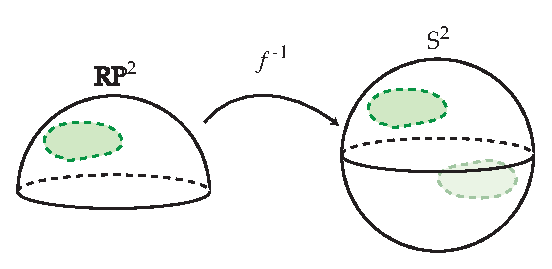
\includegraphics[width=300pt]{images/covering_spaces/rp2_quotient} \]
\end{proof}

$\RP^2$ provides us with another example of a space with a nontrivial fundamental group. From one of our theorems, we know that given $x_0\in \RP^2$ there is a bijection from $\pi_1(\RP^2,x_0)$ to $p^{-1}(\left\{x_0\right\})$ (since $\RP^2$ is simply connected), and we know that $p^{-1}(\left\{x_0\right\})$ has precisely two elements, so $\pi_1(\RP^2,x_0)\cong \Z_2$ (alternatively written by algebraists as $\Z/ 2\Z$).

\section{$\R^2 \not\cong\R^3$} 
\begin{theorem}
	$\R^2 \not \cong \R^3$
\end{theorem}
\begin{proof}
	First, recall some previous results: 
	\begin{itemize}
		\item $\R^{n+1} \setminus \{p\}$ is homotopy equivalent to $S^n$ 
		\item $\pi_1(S^2, x_0)$ is trivial 
		\item $\pi_1(S^1, x_0) \cong \Z$ 
	\end{itemize}
	
	Now suppose that $\R^2 \cong \R^3$. Then there exists some homeomorphism $h : \R^2 \to \R^3$. 
	
	Let $p \in \R^2$ and $h(p) = q \in \R^3$. Therefore $f = h|_{\R^2\setminus\{p\}} :\R^2\setminus\{p\} \to \R^3\setminus\{q\}$ is a homeomorphism. Also, from the previous results: 
	\begin{itemize}
		\item $\pi_1(\R^2 \setminus \{p\}, x_0) \cong \pi_1(S^1, y_0) \cong \Z$ 
		\item $\pi_1(\R^3, \setminus \{q\}, z_0) \cong \pi_1(S^2, w_0) \cong \{1\}$ 
	\end{itemize}
	But $f$ is a homeomorphism, so $f_* : \pi_1(\R^2 \setminus \{p\}, x_0) \to \pi_1(\R^3, \setminus \{q\}, z_0)$ is an isomorphism. However, $\Z \not \cong \{1\}$, so this is a contradiction. 
	
	Therefore $\R^2 \not \cong \R^3$, as desired. 
\end{proof}

\section{One Last Thought} 
\begin{example}
	[Not all Fundamental Groups are Abelian] Let $X = S^1 \vee S^1$ with wedge point $x_0$. Then $\pi_1(X, x_0)$ is not abelian. 
\end{example}
\begin{proof}
	Define $Y \subseteq \R^2$ as $Y = \{ (x,y) \mid x = 0 \text{ and/or } y = 0\}$.
	
	Define $\widetilde{X}$ as $Y$ with a copy of $S^1$ wedged at every $(z,0)$ and $(0,z)$ with $z \in \Z \setminus \{0\}$
	
	Define $p : \widetilde{X} \to X$ such that $(x,0)$ goes to the first copy of $S^1$ for all $x \in \R$, $(0,x)$ goes to the second, and $(z,0)$, $(0,z)$ goes to $x_0$ for all $z \in \Z$. Copies of $S^1$ wedged at $(z,0)$ go with the usual projection to the second copy of $S^1$ in $X$, and the copies wedged at $(0,z)$ go the the first copy in $X$, as shown in the image.
	
	\[
	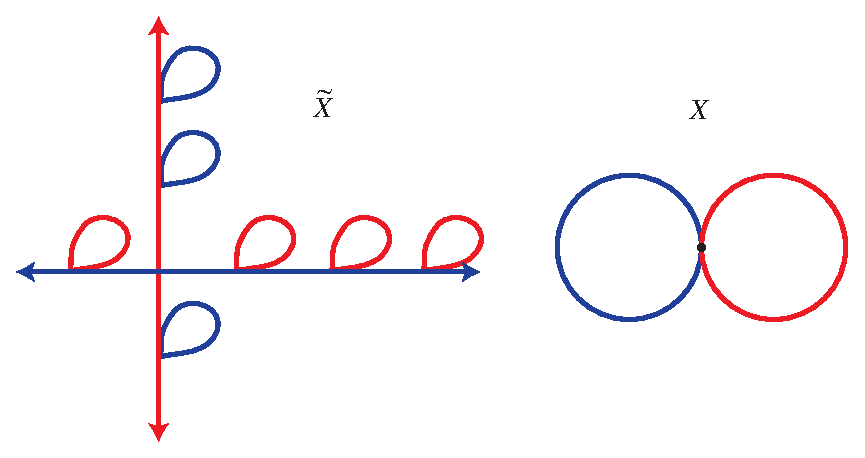
\includegraphics[width=300pt]{images/covering_spaces/nonabelian}\]
	
	Now define $\widetilde{f}(t) = (t,0)$, $\widetilde{g}(t) = (0,t)$, and $f = p \circ \widetilde{f}$, $g = p \circ \widetilde{g}$. So $f$ is a single loop on the first circle and $g$ is a single loop on the second circle.
	
	Next, lift $f * g$ and $g * f$ at the origin. The construction of $\widetilde{X}$ gives that $\widetilde{f * g}(1) = (1,0)$ and $\widetilde{g * f}(1) = (0,1)$. So, by the Monodromy theorem, as this are lifts with the same fixed point, $f * g \not \sim g * f$. Therefore $[f]$ and $[g]$ satisfy $[f],[g] \in \pi_1(X,x_0)$ and $[f][g] \neq [g][f]$, so $\pi_1(X,x_0)$ is not abelian, as desired.
\end{proof}

Well, that's everything there is to know about topology. 
